\documentclass[]{article}
\usepackage[labelfont=bf]{caption}
\usepackage[colorlinks=true,urlcolor=blue]{hyperref}
\usepackage{graphicx}
\usepackage{sidecap}
\setlength{\parindent}{0em}
\setlength{\parskip}{1em}
\begin{document}

\title{a eZ idea of inversions, part II}
\maketitle

In my \href{}{previous post} I explained my idea for why inversion polymorphisms may be common in complex plant genomes like maize. 
Here I'll describe what we're doing to start looking for them.

Inversions suppress recombination. 
The resulting lack of exchange means we expect divergence to build up between normal and inverted haplotypes, and such effects should be reflected in population genetic variability (e.g Fig. \ref{fig:fang})

\begin{SCfigure}[][h!]   
   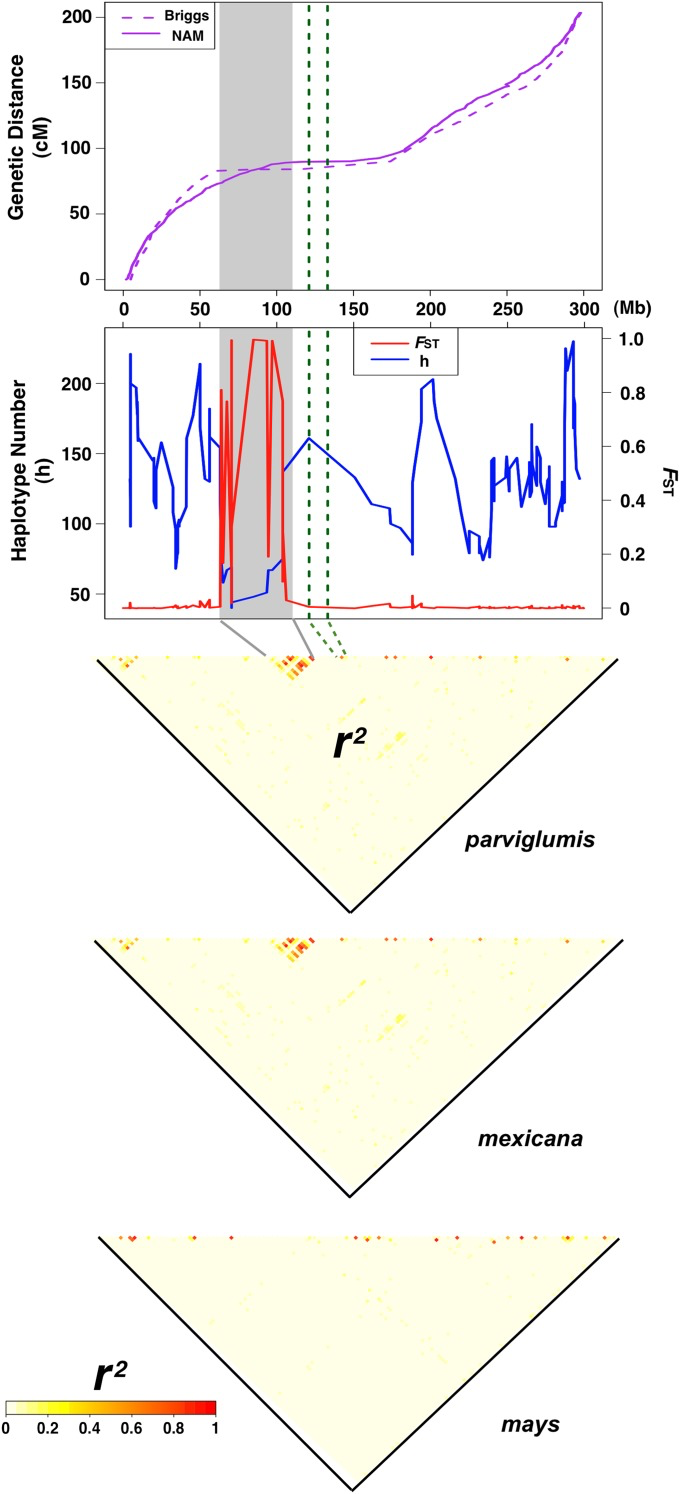
\includegraphics[width=0.3\linewidth]{/Users/jri/gdrive/fruitcase/883fig1.png}
   \caption{The impact of an inversion on diversity. Figure from \href{http://www.genetics.org/content/191/3/883}{Fang et al. 2012} showing reduced haplotype diversity, elevated $F_{ST}$ between haplotypes, increased LD, and decreased rates of crossover inside a large inversion on maize chromosome 1.} 
    \label{fig:fang}
\end{SCfigure}

I figured these effects should be reflected in a principle component analysis of diversity data from a sample segregating for an inversion.  
Indeed, when I look at \href{http://www.ncbi.nlm.nih.gov/pmc/articles/PMC3087801/}{GBS} data from several thousand maize landraces from the \href{http://seedsofdiscovery.org/maize/}{SeeDs of Discovery project}, I find my old friend \href{http://gbe.oxfordjournals.org/content/5/9/1594.full}{Inv4m} is readily identifiable (Fig \ref{fig:pcs}). 
I perform PCA on a sliding window along the chromosome, and in windows overlapping the inversion, the first principle component cleanly divides all individuals into three clusters representing the three genotypes (two homozygotes and a heterozygote) for the inversion.

\begin{figure*}[h]   
  \begin{center}
   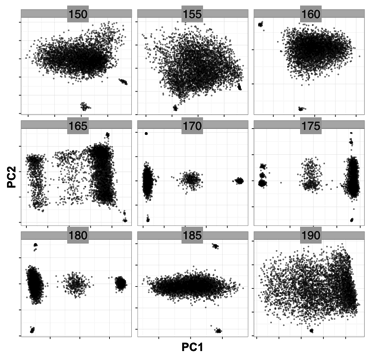
\includegraphics[width=0.7\linewidth]{/Users/jri/gdrive/fruitcase/inversions_pca.png}
   \caption{ The first two principal components of a PCA on individuals from the maize SeeDs of diversity data, plotted in 5Mb windows for part of Chr. 4. You can see a high-res version at the 1Mb scale \href{}{here}.} 
    \label{fig:pcs}
  \end{center}
\end{figure*}

So this is cool, as it hints at the possibility we may be able to use PCA to do a genome scan for putative inversions. 
I later discovered I was not alone in thinking about this possibility, but that \href{http://journals.plos.org/plosone/article?id=10.1371/journal.pone.0040224}{Ma and Amos} had suggested similar approach years ago in humans.  
The sticking point, however, was how to identify windows with putative inversions.  
Our first realization was that  scatterplots, while visually appealing,  were not very useful for classification, and that most of the time putative inversions were represented as clusters on only one of the PC's (Fig. \ref{fig:dpp}).  
This reduces the problem to one of identifying clusters of values in a single vector of data. I had \href{}{recently learned to use the DPP to estimate cluster membership}, and this seemed a similar problem. 

The DPP seems to work, and while we're still tweaking priors and testing results, it seems that using the posterior probability that there are three clusters,

\begin{equation}
\frac{P(k=3|\Theta)}{1-P(k=3|\Theta)}\div \frac{P(k=3|\Psi)}{1-P(k=3|\Psi)}
\end{equation}

where $\Theta$ is the data and $\Psi$ the prior, is a relatively simple means of identifying candidate regions that could be inversions.  
Of course even if these look real, we'll also need to convince ourselves these regions are real, and not population structure, a large indel, or some other feature of the data. 
But even a cursory glance at the data finds lots of convincing-looking regions (see Fig. \ref{fig:dpp}A) and I suspect we will find a lot of new stuff!

\begin{figure*}[h]   
  \begin{center}
   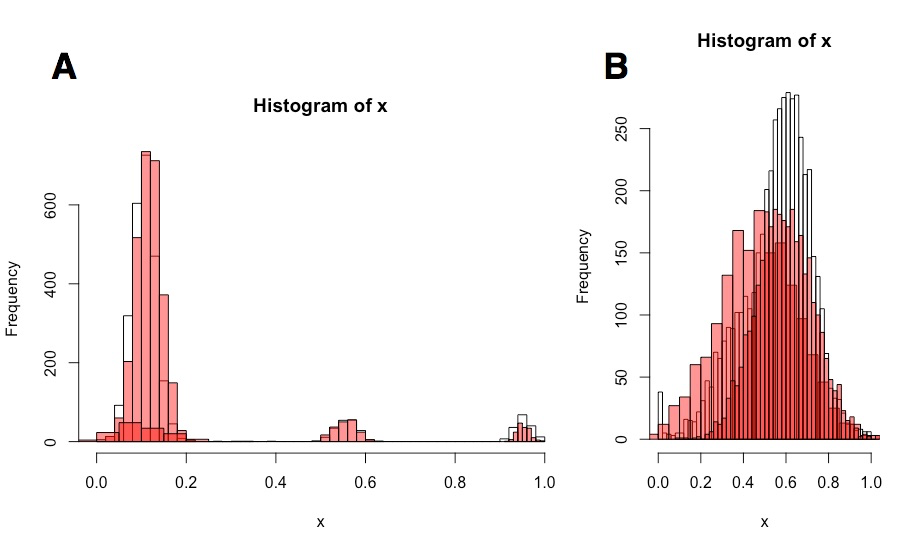
\includegraphics[width=0.7\linewidth]{/Users/jri/gdrive/fruitcase/dpp.png}
   \caption{
   Histogram of scaled [0,1] eigenvalues along an individual principal component for a particular region on chromosome 10 in the SeeDs data. The region shown in (A) appears to be consistent with an inversion polymorphism forming 3 clusteres representing the 3 genotypes at the inversion, while (B) appears a normal region of the genome lacking any evidence of an inversion.} 
    \label{fig:dpp}
  \end{center}
\end{figure*}

\end{document}